\documentclass[article,A4,12pt]{llncs}
\usepackage[T1]{fontenc}
\usepackage{amsmath}
\usepackage{amssymb}
\usepackage{amsfonts}
\usepackage{mathrsfs, bm}

\usepackage{graphicx}
\usepackage{tabularx}
\usepackage{subfig}
\usepackage{epsf,times}
\usepackage{color}
\usepackage{wrapfig}
\usepackage{cases}
\usepackage{multicol}

\usepackage[T1]{fontenc}
%\newcommand{\tmname}[1]{\textsc{#1}}
%\newcommand{\tmop}[1]{\ensuremath{\operatorname{#1}}}
%\newcommand{\tmsamp}[1]{\textsf{#1}}
%\newcommand{\tmtextsc}[1]{{\scshape{#1}}}
%\newcommand{\tmtextsl}[1]{{\slshape{#1}}}
%\newcommand{\tmtexttt}[1]{{\ttfamily{#1}}}

\leftmargin=0.0cm
\oddsidemargin=0.5cm
\evensidemargin=0.5cm
\topmargin=0cm
\textwidth=16.0cm
%\textheight=21.5cm
\textheight=20.0cm
\pagestyle{plain}
\setlength{\columnsep}{20pt}

\def\m{\mathbf{m}}
\def\H{\mathbf{H}}
\def\E{\mathbf{E}}
\newcommand{\vepsi}{{\varepsilon}}
\def\hnorm#1#2{\vert\,#1\,\vert_{#2}}
\newcommand{\R}{{\mathbb R}}
\newcommand{\Sph}{{\mathbb S}}
\def\x{\mathbf{x}}
\def\hvec{\overline{\mathbf{h}}}
\def\evec{\overline{\mathbf{e}}}

\newcommand{ \etal}{\mbox{\emph{et al. }}}

\newcommand\vect[1]{\mbf{#1}}
\newcommand{\mbf}[1]{\mbox{\boldmath$#1$}} 
\newcommand{\RC}[1]{#1 $\times$ #1 $\times$ #1}
\def\um{$\mu$m}
\def\C{$^{\circ}\mathrm{C}$}

\newcommand{\Rmnum}[1]{\expandafter\@slowromancap\romannumeral #1@}

% DEFINITION OF CUSTOM FONT SIZE
\newcommand{\customfontA}{\fontsize{50}{55}\selectfont}
\newcommand{\customfontB}{\fontsize{14.4}{20}\selectfont}
\newcommand{\customfontC}{\fontsize{30}{35}\selectfont}

\DeclareMathAlphabet{\mathpzc}{OT1}{pzc}{m}{it}

\def\clovek#1{\noindent\bgroup\vbox{\noindent#1}\egroup\vskip1em}

% TO INPUT BACKGROUND IMAGE
\usepackage{eso-pic}
\newcommand\BackgroundPic{
\put(0,0){
\parbox[b][\paperheight]{\paperwidth}{
\vfill
\centering
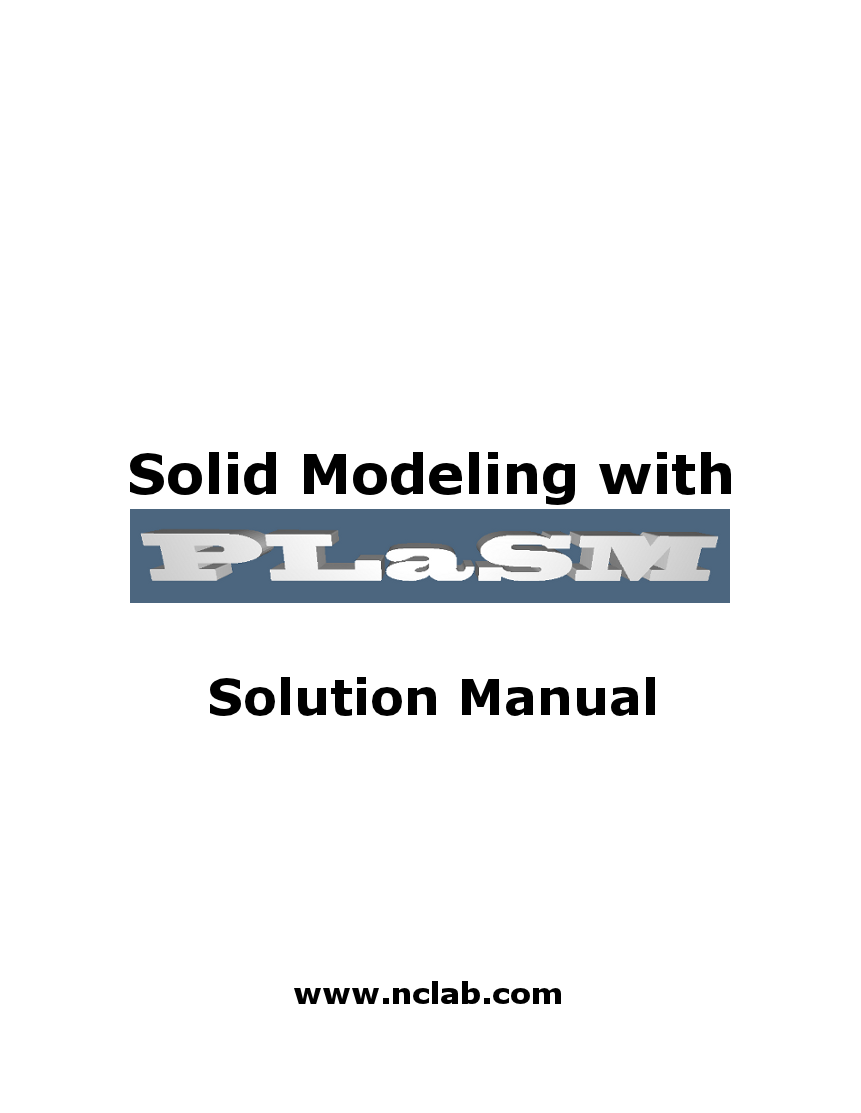
\includegraphics[width=\paperwidth,height=\paperheight]{img/plasm-solutions-frontpage.png}
%\includegraphics[width=\paperwidth,height=\paperheight]{img/background.jpg}
\vfill
}}}

%\renewcommand{\thesubsection}{(\alph{subsection})}

\begin{document}

% INPUTTING BACKGROUND IMAGE
\AddToShipoutPicture{\BackgroundPic}
\vbox{}
\pagestyle{empty}
\newpage
\textwidth=15.5cm
\ClearShipoutPicture
\newpage

%%%%%%%%%%%%%%%%%%%%%%%%%%%%%%%%%%%%%%%%%%%%%%%%%%%%%%%%%%%%%%%%%%%%%%%%%

\section*{}
\small
\subsection*{About NCLab}
Networked Computing Laboratory (NCLab) is a popular Internet-based framework for 
programming, mathematics, computer modeling, 
and scientific computing. It serves students, instructors, researchers, and the general 
public. NCLab can be used free of charge for personal non-commercial purposes such as 
private hobby or self-education, as well as for individual non-funded academic research.
All other use is subject to {\bf purchasing a license} for a symbolic fee. The fees are as low as 
\$1 per user per month for educational use, and they are used to support the development 
and operational expenses. NCLab is a product of FEMhub Inc. The name "NCLab" is 
registered with the U.S. Patent and Trademark Office (USPTO) under Trademark No. 85420518.

\subsection*{Terms of Use and Pricing}
More details on purchasing a license and using NCLab are provided in the online documents 
{\bf Pricing} and {\bf Terms of Use} that are accessible from NCLab's home page 
{\tt http://nclab.com}.

\subsection*{Contact Information}
General inquiries: {\tt info@femhub.com}\\
Sales: {\tt sales@femhub.com}\\
NCLab support: {\tt support@nclab.com}\\
Agros \& Hermes support: {\tt support@femhub.com}\\
Web page: {\tt http://femhub.com}\\
{Physical address}\\
FEMhub Inc.\\
5490 Twin Creeks Dr.\\
Reno, NV 89523

\subsection*{About This Publication}
This publication can be copied and distributed without any restrictions
as long as reference to NCLab and FEMhub Inc. is preserved.

\subsection*{Acknowledgement}
This publication features PLaSM, an open source Programming Language for 
Solid Modeling, developed by Alberto Paoluzzi, Giorgio Scorzelli, and their 
students and collaborators at the University of Rome in Italy. Some examples 
shown here come from the original PLaSM repository. Alberto's 
and Giorgio's help and support are gratefully acknowledged. 

\normalsize

\newpage
%{\ }
\setcounter{tocdepth}{2}
\tableofcontents
%\pagestyle{plain}

\newpage

\pagestyle{plain}
\setcounter{page}{1}

%%%%%%%%%%%%%%%%%%%%%%%%%%%%%%%%%%%%%%%%%%%%%%%%%%%%%%%%%%%%%%%%%%%%%%%%%

\section{Introduction}

This Solution Manual contains solutions to selected exercises from the 
PLaSM Tutorial. All models presented here are also available for 
cloning via the File Manager's Project $\rightarrow$ Clone menu.

\section{Creating Simple Objects}

\subsection{Blue Brick (A1)}

\begin{verbatim}
# Import PLaSM:
from pyplasm import *

# Define light blue color:
color = [0, 0, 1]

# Create a 3x4x5 brick:
b = CUBOID([3, 4, 5])

# Display the brick:
lab.view(b, color)
\end{verbatim}


\subsection{Red Rectangle (A2)}

\begin{verbatim}
# Import PLaSM:
from pyplasm import *

# Define light red color:
color = [1, 0, 0]

# Create a 3x1 rectangle:
r = CUBOID([3, 1])

# Display the object:
lab.view(r, color)
\end{verbatim}


\subsection{Orange Octahedron (A3)}

\begin{verbatim}
# Import PLaSM:
from pyplasm import *

# Define orange color:
color = [255/255., 140/255., 0/255.]

# Define the points:
points = [[0, -1, 1], [0, 1, 1], [0, -1, -1], [0, 1, -1], \
[2, 0, 0], [-2, 0, 0]]

# Create the convex hull:
oct = CONVEXHULL(points)

# Display the object:
lab.view(oct, color)
\end{verbatim}


\subsection{Pink Pentagon (A4)}

\begin{verbatim}
# Import PLaSM:
from pyplasm import *

# Import some things from Numpy:
from numpy import sin, cos, pi

# Define pink color:
color = [1, 0, 1]

# Number of edges on the base circle:
N = 5

# Radius of base circle:
R = 5

# Create the points:
points = []
for i in range(N):
    angle = i * 2. * pi / N
    points.append([R * cos(angle), R * sin(angle)])
    
# Create the convex hull:
penta = CONVEXHULL(points)

# View the object:
lab.view(penta, color)
\end{verbatim}


\subsection{Cyan Cone (A5)}

\begin{verbatim}
# Import PLaSM:
from pyplasm import *

# Import some things from Numpy:
from numpy import sin, cos, pi

# Define cyan color:
color = [0, 1, 1]

# Number of edges on the base circle:
N = 128

# Radius of base circle:
R = 5

# Cone height:
H = 10

# Create the points:
points = []
for i in range(N):
    angle = i * 2. * pi / N
    points.append([R * cos(angle), R * sin(angle), H])

# Add the tip (0, 0, 0):
points.append([0, 0, 0])
    
# Create the convex hull:
cone = CONVEXHULL(points)

# View the object:
lab.view(cone, color)
\end{verbatim}


\subsection{Carmine Cylinder (A6)}

\begin{verbatim}
# Import PLaSM:
from pyplasm import *

# Define carmine color:
color = [150/255., 0/255., 24/255.]

# Number of linear segments on the curved surface:
N = 128

# Radius:
R = 5

# Height:
H = 3

# Create the cylinder
cyl = CYLINDER([R, H])(N)

# View the object:
lab.view(cyl, color)
\end{verbatim}


\subsection{Topaz Tube (A7)}

\begin{verbatim}
# Import PLaSM:
from pyplasm import *

# Define topaz color:
color = [255/255., 200/255., 124/255.]

# Number of linear segments on the curved surface:
N = 128

# Inner radius:
Rin = 1.9

# Outer radius:
Rout = 2

# Height:
H = 4

# Create the tube:
t = TUBE([Rin, Rout, H])(N)

# View the object:
lab.view(t, color)
\end{verbatim}


\subsection{Sand Sphere (A8)}

\begin{verbatim}
# Import PLaSM:
from pyplasm import *

# Define sand color:
color = [238/255., 214/255., 175/255.]

# Number of linear segments on the curved surface:
N = 64

# Radius:
R = 1.0

# Create the sphere:
s = SPHERE(R)([N, N])

# View the object:
lab.view(s, color)
\end{verbatim}


\subsection{Turquoise Torus (A9)}

\begin{verbatim}
# Import PLaSM:
from pyplasm import *

# Define turquoise color:
color = [64/255., 224/255., 208/255.]

# Number of linear segments on the curved surfaces:
N = 64

# Inner radius:
Rin = 3.0

# Outer radius:
Rout = 5.0

# Create the torus:
t = TORUS([Rin, Rout])([N, N])

# View the object:
lab.view(t, color)
\end{verbatim}





\section{Transformations}

Coming soon.





\section{Binary Operations}

\subsection{Ashtray (C1)}

\begin{verbatim}
# Import PLaSM:
from pyplasm import *

# Define color:
color = [0.9, 0.9, 0.9]

# Outer cylinder:
Rout = 10.0
Hout = 3.0
cyl_outer = CYLINDER([Rout, Hout])(128)

# Inner cylinder
Rin = 8.0
Hin = 3.0
bottom_thickness = 0.5
cyl_inner = CYLINDER([Rin, Hin])(128)
cyl_inner = T(3)(bottom_thickness)(cyl_inner)

# Subtract inner cylinder from outer:
out = DIFF([cyl_outer, cyl_inner])

# Tiny cylinder to cut off the radiuses:
Rtiny = 2.0
Htiny = 2 * Rout + 2.0
cyl = CYLINDER([Rtiny, Htiny])(64)

# Lay the first cylinder horizontall over the ashtray:
cyl1 = T([3])([-Htiny/2.])(cyl)
cyl1 = R([1, 3])(PI/2)(cyl1)
cyl1 = T([3])([Rtiny + Hout/2.0])(cyl1)

# Just rotate by 90 degrees about the z axis:
cyl2 = R([1, 2])(PI/2)(cyl1)

# Cutting off the radiuses at once
out = DIFF([out, cyl1, cyl2])
 
# Display the result:
lab.view(out, color)
\end{verbatim}

\subsection{Drilled Cube (D2)}

\begin{verbatim}
from pyplasm import *
size = 2.0
radius = 0.8
color = [0.9, 0.9, 0.9]
subdiv = 64
c = CUBOID([size, size, size])
c = T([1, 2, 3])([-size/2., -size/2., -size/2.])(c)

height = size + 2.
cyl = CYLINDER([radius, height])(subdiv)
cyl = T([3])([-height/2.])(cyl)

c2 = DIFF([c, cyl])

cyl2 = R([1, 3])(PI/2)(cyl)

c3 = DIFF([c2, cyl2])

cyl3 = R([2, 3])(PI/2)(cyl)

c4 = DIFF([c3, cyl3])
\end{verbatim}


\section{Creating Simple Objects (Continued)}

Coming soon.


\section{Curves and Curved Surfaces}

Coming soon.



\section{The Power of Scripting}

\subsection{Aztec Pyramid (D1)}

\begin{verbatim}
# Import PLaSM:
from pyplasm import *

# Color:
color = [0.9, 0.9, 0.9]

# Bottom side length:
BSL = 50.0

# Top side length:
TSL = 20.0

# Height:
H = 20.0

# Number of layers:
N = 10

# Sanity checks:
ok = True
if BSL < TSL: 
    ok = False
if H <= 0:
    ok = False
if N <= 0:
    ok = False

if ok == True:
    h = H / float(N)
    e = BSL
    de = (BSL - TSL) / float(N)
    pyramid = CUBOID([e, e, h])
    for i in range(N-1):
        e -= de
        pyramid = TOP([pyramid, CUBOID([e, e, h])])
    
    lab.view(c, color)
else:
    print "Incorrect input parameters!"
\end{verbatim}

\subsection{Tower of Hanoi (D2)}

\begin{verbatim}
# Import PLaSM:
from pyplasm import *

# Color:
color = [184/255., 115/255., 51/255.]

# Bottom radius:
BR = 40.0

# Top radius:
TR = 10.0

# Height:
H = 60.0

# Number of layers:
N = 8

# Sanity checks:
ok = True
if BR < TR: 
    ok = False
if H <= 0:
    ok = False
if N <= 0:
    ok = False

if ok == True:
    # Thickness: 
    h = H / float(N)

    # Create base plate:
    plate = CUBOID([7 * BR, 3 * BR, h])

    # Create poles:
    p1 = CYLINDER([TR/3., H*1.1])(16)
    p1 = TRANSLATE([1, 2, 3])([1.5 * BR, 1.5 * BR, h])(p1)
    p2 = TRANSLATE([1])([2*BR])(p1)
    p3 = TRANSLATE([1])([2*BR])(p2)
  
    # Create the tower:
    e = BR
    de = (BR - TR) / float(N)
    tower = CYLINDER([e, h])(64)
    for i in range(N-1):
        e -= de
        tower = TOP([tower, CYLINDER([e, h])(64)])
    
    # Put the tower on the plate:
    tower = TRANSLATE([1, 2, 3])([1.5 * BR, 1.5 * BR, h])(tower)
    
    lab.view(STRUCT([plate, p1, p2, p3, tower]), color)
else:
    print "Incorrect input parameters!"
\end{verbatim}


\subsection{Horse Corral (D3)}

\begin{verbatim}
# Import PLaSM:
from pyplasm import *

# This color is called "saddle brown":
color = [139/255., 69/255., 19/255.]

# Pole width:
W = 0.2

# Pole height:
H = 2.0

# Corral radius:
r = 10.0

# Number of sides:
N = 32

# Prototype of a pole:
pole = CUBOID([W, W, H])
pole = T([1, 2])([-W/2., -W/2.])(pole)
pole = T([1])([r])(pole)
 
# Create all poles:
angle = 2 * PI / N
fence = []
for i in range(N):
    fence.append(R([1, 2])(i * angle)(pole))
    
# Prototype of horizontal logs:
from numpy import sin, cos
L = 2 * r * sin(angle / 2)
log = CUBOID([0.05, L, 0.2])
log = R([1, 2])(angle/2)(log)
log = T([1, 3])([r, H/8.])(log)  
log2 = T([3])([H/4.])(log)
log3 = T([3])([H/4.])(log2)

# Append horizontal logs to each pair of 
# adjacent poles:
for i in range(N):
    fence.append(R([1, 2])(i * angle)(log))
    fence.append(R([1, 2])(i * angle)(log2))
    fence.append(R([1, 2])(i * angle)(log3))

# Show the complete fence:
lab.view(STRUCT(fence), color)
\end{verbatim}

\subsection{Wagon Wheel (D4)}

\begin{verbatim}
Coming soon.
\end{verbatim}

\end{document}
